\documentclass{article}
\usepackage{outline}
\usepackage{float}
\usepackage{graphicx}
\usepackage{color}
\usepackage{amsmath}
\usepackage{cite}
\graphicspath{ {Figs/} }

\begin{document}

 \title{Multiscale Modeling of the Paradoxical Roles of the Immune System in EMT-Mediated Cancer}
 \maketitle

\section*{Abstract}
%% Basic Introduction (1-2 sentences)
During tumorigenesis and throughout the lifetime of a tumor, the immune system is constantly engaged in complex interactions in and around the tumor.
%% More Detailed Background (2-3 sentences)
These interactions are influenced by the tumor microenvironment (TME) and in particular by the cellular process of epithelial-to-mesenchymal transition (EMT) in an as-yet unexplained manner.
In turn, both the tumor and the immune system exert substantial influence over the TME in competition to influence the fate of the host.
%% General Problem (1 sentence)
Determining the critical factors and mechanisms involved remains a crucial task for cancer immunotherapy.
%% Summarizing Main Result (1 sentence)
Here, we seek to understand how interplay between the tumor, the immune system, and EMT can determine the outcome of cancer.
%% The Main Result (2-3 sentences)
We developed a multiscale agent-based model that describes tumor-immune interactions and how EMT modulates these.
Exploration of the model revealed that increasing the growth arrest of mesenchymal cells in some circumstances results in a more tumor-friendly environment and sometimes less.
In contrast, enhancing the immune evasiveness of mesenchymal cells always leads to a more tumor-friendly microenvironment.
Moreover, encouraging the TME towards a pro-EMT state also benefits the tumor.
%% Putting into a More General Context (1-2 sentences)
Together, these results indicate that the joint regulation of the TME by the immune system and the tumor itself provides possible targets for future cancer therapies, in particular cancers such as pancreatic cancer in which EMT is speculated to play a role.

%%%%%%%%%%%%%%%%%%%%%%%
%                    INTRODUCTION                    %
%%%%%%%%%%%%%%%%%%%%%%%

\section{Introduction}
Immunotherapy is slowly revolutionizing how we treat cancer.
Year-by-year, new breakthroughs in the field produce new, effective drugs and therapies that have a significant impact on patient health and survival\cite{pardoll2012blockade}\cite{restifo2012adoptive}.
% A More examples? Reviews or non-reviews? Explain some of the examples?
%AM I will add a few 
There are myriad untapped avenues by which scientists can further explore the role of the immune system in regulating and combatting cancer; in addition to direct cell-cell interactions between immune and cancer cells, the means by which immune cells interact with and modulate the tumor microenvironment (TME) is an important research area. Immune cells can be understood as one constituent of the TME: responding to the environment's inflammatory signals, fighting the mutated cells present, and then restoring homeostasis in that local context\cite{de2006paradoxical}.
Understanding each step in this immune cascade in the context of the TME will be necessary in order to fully explore and exploit all options of immunotherapy.

Recent work on cancer-immune interactions has shown that the inflammatory conditions of the TME can play large and sometimes surprising roles in tumor growth.
Guo describes a model in which the inflammatory state of the TME affects the cell cycles of the stem cells by increasing proliferation, decreasing apoptosis, and enhancing DNA damage that leads to mutations\cite{guo2017multiscale}.
Guo uses the model to show that while inflammation does have an oncogenic effect, it can also have an onco-protective role as periods of mild inflammation are better at preventing cancer than periods of no inflammation in patients that have intermittent bouts of severe inflammation.
However, the aspect of the model that included the immune system was minimal: regardless of the inflammatory environment, any cells with sufficient pathway mutations (2 in their model) had a fixed probability of being cleared by the metabolism-immune balance response. 
In this paper, we hope to improve the model by including a more robust immune module and exploring how this axis will improve our understanding of inflammatory effects on the tumor.
In addition, we explore an extra component of Guo's stem cells: where they lie on the epithelial-mesenchymal axis.
So, in total, we will explore the joint interactions of the tumor, the immune system, and the epithelial-mesenchymal spectrum.
We will also study the effects of the TME on these interactions.

The tumor interacts with the immune system by initiating the sequence of events that results in the activation of the adaptive immune response.
It accomplishes this by presenting antigens that innate immune cells recognize and carry to lymph nodes to activate, among other things, T cells.
Also, tumor cells engage in certain cellular processes that shape the TME and thus impact the immune system.
In particular, tumor cells release transforming growth factor beta (TGF-$\beta$) that creates a tumor-supportive environment by shifting the immune balance to being immunosuppressive via enhancing activation of Treg cells.

This particular cytokine is also a driver of the epithelial-to-mesenchymal transition (EMT) and through generating TGF-$\beta$ the tumor creates a more mesenchymal phenotype within the TME.
In this way, the tumor shifts the balance of local environment along the EMT spectrum.

The immune system has several competing interactions with the tumor.
While the cytotoxic immune cells, NKs and cytotoxic T cells (CTLs), seek out and lyse tumor cells, the regulatory branch of the immune system, which will be accounted for by Tregs in our model, slows down the effector functions of these other cells.

In relation to EMT, the Tregs of the immune system drive the EMT process by releasing TGF-$\beta$ upon arriving at the tumor site\cite{terry2017new}.
In this way, just as the tumor cells push the TME towards a mesenchymal phenotype, so too do the Tregs.

Epithelial-to-mesenchymal transition (EMT) describes the (reversible) cell plasticity process by which epithelial cells transition into mesenchymal cells.
While the epithelial cells often stay bound together in layers, mesenchymal cells have gained motility and even stem-like properties\cite{nieto2016emt}.
They have thus become a subject of great interest in cancer research having been connected to tumor initiation, progression, and metastasis\cite{nieto2016emt}.
There are many other characteristics distinctive of mesenchymal cells and still much research being done in further quantifying these and determining others.
Of interest to us, the literature reveals two qualities of mesenchymal cells that are particularly relevant in the context of cancer and the immune system.
The first is that mesenchymal cells are less susceptible to immune clearance\cite{terry2017new}. 
%
The second is that mesenchymal cells proliferate at a slower rate. Ref
 %A Adam said he had a reference in mind for this.

The research on mesenchymal cells' immune evasiveness is quite conclusive with the research even going so far as establishing functional causes for this phenomenon.
As a cell is being targeted by cytotoxic immune cells for clearance, a physical connection between the two cells must be created in order to precipitate the lysing event.
This immunological synapse, however, is dependent upon the surface proteins of the target cell, and in the case of mesenchymal cells there is preliminary evidence that these surface markers are down-regulated in such a way that the immune synapse is more difficult to form\cite{terry2017new}.
There are also other structural changes that take place in mesenchymal cells that could contribute to this refractory nature towards immune clearance.
Regardless, the evidence currently demonstrates a ``slipperiness'' of mesenchymal cells in regards to immune lysing that in our model we will refer to as mesenchymal immune evasion, or MIE.

The other facet of mesenchymal cells of importance in this research is their slower proliferation rate, and this is tied to the observation that mesenchymal cells often express a more stem-like phenotype.
Indeed, even in healthy tissue, this is readily observed and seen as a useful mechanism for homeostasis as epithelial cells can transition to mesenchymal, stem-like cells under appropriate conditions. Ref
While many qualities are associated with being stem-like, we choose to focus on a reduced proliferation rate. Ref
Cancer cells are well-known for achieving unregulated proliferation, so exploring a subset of cancer cells with decreased proliferation could provide intriguing new results.
In our model, we refer to this property as mesenchymal growth arrest, or MGA.

In the following sections of the paper we first introduce the model modularly, which is appropriate given its multiscale and hybrid nature.
We then perform sensitivity analysis and identify parameters that are crucial for the progression to tumorigenesis.
We analyze the competing effects of EMT and of the immune system on tumorigenesis and find that EMT intricately regulates tumorigenesis: under certain regimes a careful balance of EMT- and immune-driven process can significantly prolong cancer-free survival.


%%%%%%%%%%%%%  INTRO PARAGRAPH GRAVEYARD %%%%%%%%%%%%%%%%

%They release cytokines that alter the extracellular matrix, promote angiogenesis, and create an inflammatory environment.
%This last one, in particular, results in the impairment of cytotoxic capabilities of immune cells.
%Through 
%
% its presence and by the cellular processes it engages in that result in shaping the TME.
%On the one hand, the mutated DNA of tumor cells results in these cells being recognized as foreign by members of the innate immune system such as natural killer (NK) cells and dendritic cells.
%It is then these cells that initiate the cascade of cytokines that result in the full activation of the body's immune system to fight the non-self cells.
%On the other hand, the tumor cells actively work to shape the immune response that the body launches.
%This is accomplished through its own set of cytokines, such as transforming growth factor beta (TGF-$\beta$), that work to create a tumor-supportive environment, including shifting the immune balance to be immunosuppressive by enhancing the recruitment of Treg cells. Since TGF-$\beta$ is also a driver of EMT, then through direct release of TGF-$\beta$ and recruitment of TGF-$\beta$-secreting Treg cells, cells of the tumor and the surrounding tissue are driven towards a more mesenchymal profile. 

%In quantifying this property, we use the model parameter `mesenchymal growth arrest', MGA.
%This choice is less about associating this property with quiescence and more about creating a simple name that easily, if not roughly, captures the essence of what is being modeled.
%For example, while mesenchymal proliferation reduction might be a more accurate term, thinking in terms of a negative formulation adds one additional twist to accurately interpreting results which we felt was more detrimental than the possible confusion of invoking ``quiescence.''

%This plays an important yet complicated role in tumor initiation, progression, and metastasis\cite{nieto2016emt}. % References more specific to this claim might be in this paper's references. 
%As mesenchymal cells often exhibit stem-like properties, their existence in a tumor has been tied to the initiation and progression of cancer\cite{nieto2016emt}. % References more specific to this claim might be in this paper's references.
%Also, due to their motility, some have viewed them as a natural precursor to metastasis\cite{alderton2012metastasis}. 
%
%Conversely, the mesenchymal cells in the tumor downregulate certain surface markers making it more difficult for cytotoxic immune cells to form the immune synapse necessary to lyse the cancer cell\cite{terry2017new}.
%Taking these three aspects together, all influencing the others, we can consider the simple diagram in Figure \ref{fig:3PartFig} and see just how much potential there is for exploring all these relationships.
%Each of these three pieces will be briefly explored in turn for how they will influence one another.









%%%%%%%%%%%%%%%%%%%%%%%
%                         METHODS                        %
%%%%%%%%%%%%%%%%%%%%%%%


\section{Methods}
To address the questions around the relationships among cancer, the immune system, and EMT, we extended the multiscale, agent-based model of Guo to include an immune module and an EMT axis for the tissue cells.
The agents in the model are the tissue cells with tumorigenic potential.
They can either be mutation-free, or have any combination of three possible pathway mutations.
We model the immune cells as discrete variables but as one collective, in other words they are not agents themselves.
The cytokine TGF-$\beta$ is a continuous variables within the tumor microenvironment (TME).
It is worth noting that there is no spatial aspect to this model.
In doing this, we are assuming that cells are well-mixed as are all the relevant cytokines and other molecules acting on the system.
Finally, tissue cells can be labeled either epithelial or mesenchymal, and this labeling can change over time and depends both on the TME and the internal workings of each individual cell.

\subsection{Tissue Cells}\label{TissueCells}
The tissue cells at all times have associated with them two important quantities: which combination of mutations they carry and an EMT score.
The model has three pathways that have the potential to mutate over the course of a simulation.
There is a proliferation pathway that when mutated increases the probability of the cell proliferating.
There is an apoptosis pathway that when mutated decreases the probability of the cell undergoing apoptosis.
There is an immune evasion pathway that when mutated decreases the probability that an immune cell can effectively clear the mutated cell.
% It might be nice to have a table to summarize this information?
The EMT score will be exposited in Section \ref{EMT}. % make sure this is really the best decision


%Add differential equations? % Should this be done here or where I have it later?

\subsection{The Immune System}\label{ImmuneSystem}
The immune system is modeled as having three active immune cell types: NKs, CTLs, and Tregs.
The NKs and CTLs act on the system by recognizing mutated cells and clearing them.
% A Should this be justified here or mentioned in the intro?
% AM: justifed no; Intro yes
Upon successful clearance, they themselves are then deactivated and removed from the immune population.
%
Tregs act on the system by suppressing the effector functions of NKs and CTLs, making it less likely they can clear mutated cells.
In addition to this, Tregs release TGF-$\beta$ which further shapes the TME by pushing tissues cells more towards a mesenchymal phenotype.

\subsection{EMT}\label{EMT}
Each tissue cell has an EMT score between 0 and 1.
When the score is above a fixed threshold value, the cell is labeled as mesenchymal.
Otherwise, it is below the threshold and labeled as epithelial.
For the purposes of the model, a cell in an epithelial state is considered in the base state, and one in a mesenchymal state will have some of its parameters updated.
In particular, mesenchymal cells benefit from increased immune evasion but suffer from decreased proliferation.
Note, that because the immune system can only clear mutated cells, the increased immune evasion only benefits mutated mesenchymal cells.

\subsection{Model Simulation}

\subsubsection{Initial conditions} Every model run starts with a fixed amount of cells, $N_0$.
However, different parameter values will lead to different steady states for the population of tissue cells.
In light of this, a warmup period of ~1000 cell cycles is used in which time no mutations are allowed to happen.
Thus, the only immune cell present is NKs.
After the warmup cycles are complete, a mutagenic event is simulated in which all the tissue cells experience a random increase in their probability to mutate.
From then on, a cell which proliferates either mutates or increases its probability of mutating later on.

\subsubsection{Tissue cell fate}
During each cell cycle, every cell randomly is assigned a cell fate from the following options:
\begin{itemize}
\item proliferation
\item apoptosis
\item immune clearance (by NKs or CTLs)
\item rest in $G_0$ %A use both here? - % AM: change to 'rest in' everywhere
\end{itemize}

For each cell, a weight is chosen for each option and these are normalized to probabilities which then are used to randomly determine what each cell does during the cell cycle.

\paragraph{Proliferation}
There are four factors that contribute to the probability that a cell will proliferate.
The first is a base proliferation probability that all cells have, $p$.
Second, if the cell has a mutation in the proliferation pathway, then the weight for proliferation is proportionally increased by $\text{prolif}_{\text{up}}$.
Third, if the cell is mesenchymal, then the weight for proliferation is proportionally decreased by $m_{GA}$, which stands for mesenchymal growth arrest.
Fourth, there is a negative feedback of the cells on their own proliferation which is quantified by a Hill factor.
In total, the weight for proliferation is given by

$$ p_{\text{prolif}} = p(1+\delta_{\text{PM}}\text{prolif}_{\text{up}})(1-\delta_{MES}m_{GA})\frac{N_0}{N_0+N} $$

\paragraph{Apoptosis}
There are two factors that contribute to a cell's weight for undergoing apoptosis.
There is a basal apoptosis rate that all cells experience, $d$ for death.
Second, if the cell has a mutation in the apoptosis pathway, then the weight for undergoing apoptosis is proportionally decreased by $\text{apop}_{\text{down}}$.
In total, the weight for apoptosis is given by 

$$ p_{\text{apop}} = d(1-\delta_{\text{AM}}\text{apop}_{\text{down}}) $$

\paragraph{Immune Clearance}
For both NK clearance and CTL clearance, the weights are built with the same factors but have different parameter values for NK and CTLs.
First of all, the cell needs to be mutated, $\delta_M$.
Second, there is a Hill factor that captures the probability of an immune cell finding and interacting with the given tissue cell.
Third, NKs and CTLs have their own efficacy parameters, $E_{\text{NK}}$ and $E_{\text{CTL}}$, which can be understood as the weight for immune clearance given an immune cell has found the mutated cell.
Fourth, there is a decreasing Hill factor based on the number of Treg cells present.
Finally, there are two factors that proportionally decrease the weight of immune clearance depending on if the cell has an immune evasion mutation or if it is mesenchymal.
In total, the weight of NK clearance is given by

$$ p_{\text{NK}} =\delta_M \frac{\text{NK}}{N/N_{1}+\text{NK}}  \frac{E_{\text{NK}}}{1+\text{Treg}/\text{Treg}_{\text{EC50}}} (1-\delta_{IEM}\text{IE}_{\text{up}})(1-\delta_{MES}m_{\text{IE}}) $$
%$$\qquad\qquad \qquad(1-\delta_{IEM}\text{IE}_{\text{up}})(1-\delta_{MES}m_{\text{IE}})$$
% Should I worry about the order in which these appear? Rearranging would make the formula look better, but the order I have introduced them makes the most sense.
% Also, any thoughts on NK, CTL, Treg not being italicized? While other capital letters are?

A similar formula holds for CTLs with only the number of CTLs and their efficacy being different from the above equation.


\paragraph{Rest in $G_0$} %A use both for this section heading?
The weight associated with quiescence is taken as 1 except in the case of Mesenchymal cells.
For Mesenchymal cells, the weight lost to proliferation is added to the weight of quiescence.
Hence, the weight of quiescence is given by

$$ p_{rest} = 1 + \delta_{\text{MES}}p(1+\delta_{\text{PM}}\text{prolif}_{\text{up}})m_{GA}\frac{N_0}{N_0+N} $$ 
%YA style choice: p_{G_0},p_{rest},p_{\text{rest}},p_{GA}???

The reason for adding that term is due to the understanding that overall mesenchymal cells proliferate less as individual cells remain longer in the $G_0$ phase. %YA is this the right way to word this?

\subsubsection{Completing the Cell Cycle}
After the cell fates are determined and the results reflected in the system, there are a few things that happen before the system moves on to a new cell cycle.
First, the NK and CTL populations are reduced by the number of mutated cells they cleared.
% A Similar to previous comment: should I cite reference for this here or put this up in the intro?
% AM no need for extra here: just in intro
This represents the fact that individual immune cells lose efficacy as they carry out their effector functions. 
%
All proliferating cells have a nonzero probability of undergoing a pathway mutation.
If they do, one is randomly chosen among the three and that one either mutates or remains mutated.
% A Updated this after Adam had question. Does this make sense as is?
% AM I don't understnad 'remains mutated'
If the cell does not undergo a mutation, then its probability of mutation during subsequent cell increases. 
%
Then, the EMT values for each cell is updated.
This depends on the cells current EMT score and how much TGF-$\beta$ is currently in the system.
Each cell receives an amount of TGF-$\beta$ given by

$$ \text{TGFB}_i = \text{TGFB}/N + X_i, \quad X_i \sim N(0,\sigma^2)$$

where $\sigma$ is a parameter in the model.
If this quantity is large enough, relative to the EMT score of the cell, then the cell will undergo EMT and its EMT score will increase.
If not, then the cell undergoes the reverse process, MET, and its EMT score will decrease.
Each cell then is relabeled as either epithelial or mesenchymal depending on its new EMT score and whether it is below or above the mesenchymal threshold.




\emph{Adam, if you're just reading the PDF, then know that I'm really not sure if this next paragraph belongs in the paper.}

%%%%%%%%%	I think this next section is too much detail that just confuses the reader. I don't think I need to explain my implementation, just the process. Thoughts?	%%%%%%%%%%%%%%%%%%%%
% AM: yes, remove or shorten to one sentence at end of previous para.
This quantity is then compared to $2-\text{EMT}_i$ where $\text{EMT}_i$ is the EMT score of the $i^{th}$ cell on a scale of $[0,1]$ with $0$ representing most epithelial and $1$ representing most mesenchymal.
If $\text{TGFB}_i>2-\text{EMT}_i$, the cell becomes more mesenchymal and will have a higher EMT score.
If $\text{TGFB}_i<2-\text{EMT}_i$, the cell becomes more epithelial and will have a lower EMT score.
The reason for the expression $2-\text{EMT}_i$ can be understood this way: 
the bounds on the EMT score guarantee $2-\text{EMT}_i\in[1,2]$.
Hence, there either needs to be a lot of TGF-$\beta$ in the system or a large amount of randomness for a cell to undergo EMT.
In addition, a cell having a higher EMT score will have a higher chance of continuing in the EMT process whereas a cell low on the EMT spectrum will have a higher chance of moving towards a more epithelial phenotype.
%%%%%%%%%%%%%%%%%%%%%%%%%%%%%%%%%%%%%%%%%%%%%%%%%%%%%%%




Next, the amount of TGF-$\beta$ for the next cell cycle is determined by the number of mutated cells and the number of Treg cells, each one producing a fixed amount of TGF-$\beta$. It is given by

$$ \text{TGFB}_k = \text{tgfb}_{\text{mut}}M_k + \text{tgfb}_{\text{Treg}}\text{Treg}_k$$ % clear that M is number of mutants, right?

Finally, the immune populations are updated.
For the NKs, they obey the following differential equation:
 
$$ \text{NK}' = \sigma_{\text{NK}} - d_{\text{NK}}\text{NK} $$

which is discretized to

\emph{Adam, if you are reading the PDF, you will see the same equations multiple times as I figure out which one I like best.}

%%% I like the first of these two options. You set aside the amount you know you will gain (sigma/d) and then let the rest decay exponentially
% AM yes first one 
$$ \text{NK}_{k+1} = \left (\text{NK}_k-\frac{\sigma_{\text{NK}}}{d_{\text{NK}}} \right )\exp(-d_{\text{NK}}\Delta t)+\frac{\sigma_{\text{NK}}}{d_{\text{NK}}} $$

%%% For this one, the initial decays exponentially and then you add some fraction of sigma/d depending on how big your time step is
$$ \text{NK}_{k+1} = \text{NK}_k\exp(-d_{\text{NK}}\Delta t)+\frac{\sigma_{\text{NK}}}{d_{\text{NK}}} \left(1-\exp(-d_{\text{NK}}\Delta t)\right)$$
%%% The first one is better though in my opinion.

% For all 3 discretizations of immune cell dynamics, I could create a quantity R_* (for recruitment? maybe better letters exist) so the formula would be 
% *_{k+1} = (*_k-R_*)\exp(-d_*\Delta t)+R_*,\quad R_*=\frac{\sigma_*}{d_*}
%% Option 1b from above:
$$\text{NK}_{k+1} = (\text{NK}_k-R_\text{NK})\exp(-d_\text{NK}\Delta t)+R_\text{NK},\quad R_\text{NK}=\frac{\sigma_\text{NK}}{d_\text{NK}}$$





%%%% Which of these two paragraphs is better? Currently the intro does not mention APCs and I don't think I need to go into that, especially when APC_k = \tilde{M}_k
For CTLs and Tregs, they rely on mutant cells being cleared before they can be activated.
Let $\tilde{M}_k$ represent the number of mutant cells cleared by the immune system during cell cycle $k$.
In addition, Treg recruitment is upregulated by TGF-$\beta$, which will be incorporated via a Hill function.
We choose the following differential equations to govern the CTL and Treg populations:

\begin{align*}
\text{CTL}' & = \sigma_{\text{CTL}}\tilde{M} - d_{\text{CTL}}\text{CTL} \\
\text{Treg}' & = \sigma_{\text{Treg}}\tilde{M} \frac{\text{TGFB}}{1+\text{TGFB}/\text{EC50}}- d_{\text{Treg}}\text{Treg}
\end{align*}

Discretized, these are:

\begin{align*}
\text{CTL}_{k+1} & = & \left (\text{CTL}_k-\sigma_{\text{CTL}}\tilde{M}_k/d_{\text{CTL}}\right )\exp(- d_{\text{CTL}}\Delta t) + \sigma_{\text{CTL}}\tilde{M}_k/d_{\text{CTL}}\\
\text{Treg}_{k+1} & = & \left (\text{Treg}_k-\frac{\sigma_{\text{Treg}}\tilde{M}_k}{d_{\text{Treg}}} \frac{\text{TGFB}}{1+\text{TGFB}/\text{EC50}}\right )\exp(-d_{\text{Treg}}\Delta t)+\\
& & \frac{\sigma_{\text{Treg}}\tilde{M}_k}{d_{\text{Treg}}} \frac{\text{TGFB}}{1+\text{TGFB}/\text{EC50}}
\end{align*}

%% Or using R_*
\begin{align*}
\text{CTL}_{k+1} & =\left (\text{CTL}_k-\tilde{M}_kR_{\text{CTL}}\right )\exp(- d_{\text{CTL}}\Delta t) + \tilde{M}_kR_{\text{CTL}}\\
\text{Treg}_{k+1} & =\left (\text{Treg}_k-\tilde{M}_kR_{\text{Treg}}\right )\exp(-d_{\text{Treg}}\Delta t)+\tilde{M}_kR_{\text{Treg}}
\end{align*}
where
\begin{align*}
R_{\text{CTL}} &= \sigma_{\text{CTL}}/d_{\text{CTL}}\\
R_{\text{Treg}} &=\frac{\sigma_{\text{Treg}}}{d_{\text{Treg}}} \frac{\text{TGFB}}{1+\text{TGFB}/\text{EC50}}
\end{align*}
%% End of option 1

%% Beginning of option 2
For CTLs and Tregs, however, they rely on antigen presenting cells (APCs) to be activated, and these APCs in turn rely on mutated cells being cleared so that they can bind antigens.
In addition, Treg recruitment is upregulated by TGF-$\beta$, which will be incorporated via a Hill function.
Thus, let $\text{APC}$ represent the number of mutated cells cleared by the immune system during a given cycle.
We choose the following differential equations to govern the CTL and Treg populations:

\begin{align*}
\text{CTL}' & = \sigma_{\text{CTL}}\text{APC} - d_{\text{CTL}}\text{CTL} \\
\text{Treg}' & = \sigma_{\text{Treg}}\text{APC} \frac{\text{TGFB}}{1+\text{TGFB}/\text{EC50}}- d_{\text{Treg}}\text{Treg}
\end{align*}

Discretized, these are:

\begin{align*}
\text{CTL}_{k+1} & = & \left (\text{CTL}_k-\sigma_{\text{CTL}}\text{APC}_k/d_{\text{CTL}}\right )\exp(- d_{\text{CTL}}\Delta t) + \sigma_{\text{CTL}}\text{APC}_k/d_{\text{CTL}}\\
\text{Treg}_{k+1} & = & \left (\text{Treg}_k-\frac{\sigma_{\text{Treg}}\text{APC}_k}{d_{\text{Treg}}} \frac{\text{TGFB}_k}{1+\text{TGFB}_k/\text{EC50}}\right )\exp(-d_{\text{Treg}}\Delta t)+\\
& & \frac{\sigma_{\text{Treg}}\text{APC}_k}{d_{\text{Treg}}} \frac{\text{TGFB}_k}{1+\text{TGFB}_k/\text{EC50}}
\end{align*}
%% End of option 2





\subsubsection{Progression and tumorigenesis}
At the end of each cell cycle, the proportion of tissue cells that are mutated is calculated, and if it is above a certain threshold, a tumorigenic event is recorded and the patient is determined to have cancer (using a similar strategy to Guo).
The Time to Cancer is given as the time from the start of the simulation, not including warmup, until tumorigenesis.
Simulations run until either a tumorigenic event is recorded or until the maximum number of cycles has been reached.
%It is also possible with the right combination of parameters, to have patients run out of cells entirely.
%The model does not distinguish between these patients and those that have a cancer diagnosis.
%The reason is that these patients have succumb to some combination of inflammatory and mutagenic events.





%%%%%%%%%%%%%%%%%%%%%%%
%                          RESULTS                         %
%%%%%%%%%%%%%%%%%%%%%%%

\section{Results}

\begin{figure}[H]
\center
\frame{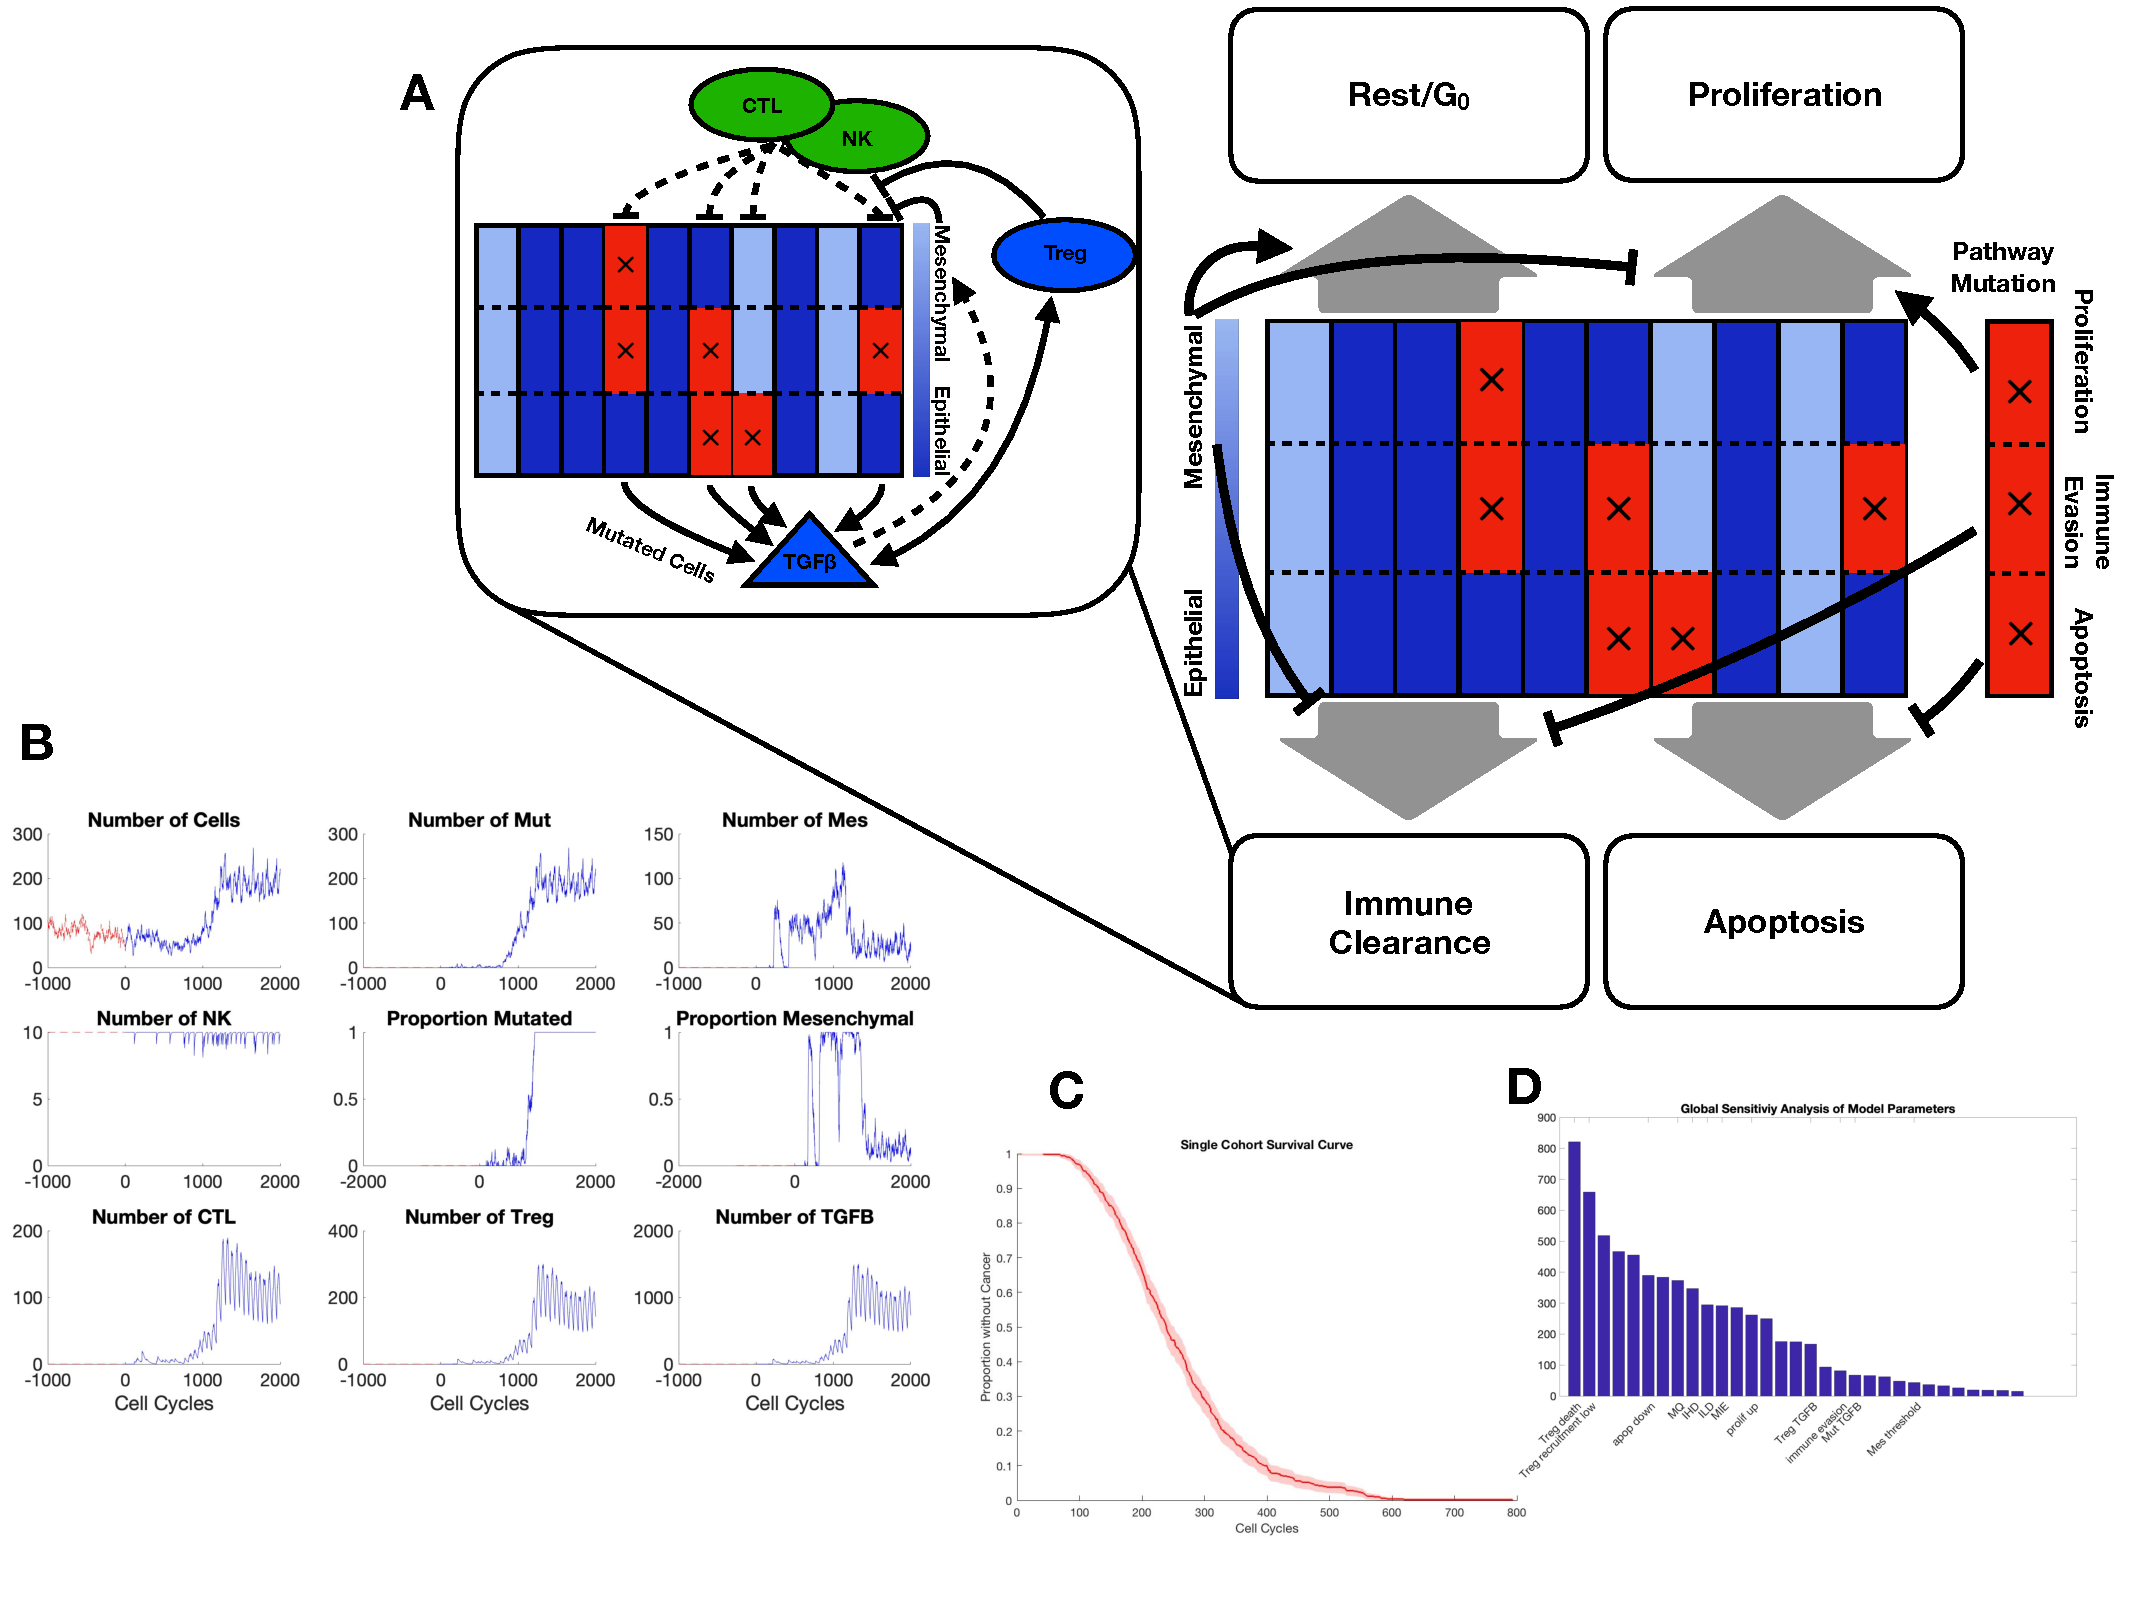
\includegraphics[width=\columnwidth]{Figure1/Figure1.pdf}}
\caption{A. Schematic depiction of the model with blue/red denoting non-mutated/mutated cells in the agent-based model. In each cycle, the fate of a cell is regulated by the EMT state of the cell and by any pathway mutations harbored. Inset shows major processes of immune system regulation on the tissue cells.
B. Example simulation of the dynamics of a one patient; warmup period is shown in red.
The inflammation cycling scheme is graphically represented above the patient dynamics.
C. Example survival curve for one cohort of patients with basal parameter values.
%A Should I list out all parameter values? A subset? Or refer to supplement for base parameter values?
D. Global sensitivity analysis of model parameters using the Morris one-step-at-a-time method.}
\label{fig:ModelIntro}
\end{figure}

\subsection{Exploring the Model}\label{ExplModel}
In Figure \ref{fig:ModelIntro}A a schematic description of the model is shown.
% A It seems the rest of this paragraph belongs in the Methods section, yeah?
% AM : yes
Here, each cell is represented as a column with three components representing the three possible mutations a cell can have.
If the component is red and has an `X' in the middle, then that indicates the cell has undergone a pathway mutation corresponding to the annotation to the right of the cell block.
Any cell that has a pathway mutation is counted as a mutated cell and contributes towards the total number of cancer cells.
The EMT score of each cell (denoting position along the EMT spectrum) is associated with a color given by the legend to the left of the cell block. 
In the model the EMT score is continuous but the labeling of epithelial or mesenchymal is a binary determined by being below or above a threshold.



% A This next commented out paragraph seems to belong somewhere, but where? I would think in the Intro.
% AM: yes in intro

%While biologically, there may be only a few discrete stable cell states available on the EMT spectrum, recent studies highlight a growing number of states accessible, with research indicating there are several equilibria along the spectrum\cite{hong2015ovol2}.
%In our model, this is actually just a binary and that is why the cells shown are at one extreme or the other of the spectrum.



In the right half of Figure \ref{fig:ModelIntro}A one can see the cell cycle choices that each cell will make each cell cycle.
These are the four thick, gray arrows.
Each of the cells will choose which arrow to follow each cell cycle, and this decision is influenced by the properties of the cell as well as external factors like the immune system and the TME.
The inset on the left gives an overview of how the immune system works.
The dashed arrows indicate that the action is probabilistic rather than deterministic.
In other words, the cytotoxic cells will randomly clear some subset of mutated cells and TGF-$\beta$ increases the probability of cell transitioning or staying in a mesenchymal state.

For a typical {\it in silico} patient, see Figure \ref{fig:ModelIntro}B.
The inflammation cycling scheme shown at the top of Figure \ref{fig:ModelIntro}B is repeated throughout.
We will return to this shortly.
It is at cell cycle number 541 the proportion of mutated cells reaches 50\% and so the patient has a Time to Cancer of 541, or 405.75 days. 
At the same time as mutated cells are taking over, most cells are transitioning to a mesenchymal phenotype.
After the Time to Cancer, the mutated cells continue their rapid growth and soon make up 100\% of the cells.
Meanwhile, all the cells become mesenchymal for a short duration before most transition back to an epithelial state.
% Once the Time to Cancer has been determined for a patient, most simulations shown later stop. [??? mean to say: we stop the simulation?]
%We do this because once such a high proportion of cells have mutated, the mutant cells quickly take over and make up 100\% of all cells.

Considering the immune populations, notice that the NK population basically stays constant while the lymphocyte populations quickly dwarf the NK population once cells begin to mutate.
These lymphocyte populations appear to exhibit oscillatory behavior, however this is not due to intrinsic dynamics but rather due to the inflammation scheme that this patient is undergoing: 
the patient alternates between 30 cell cycles of high inflammation and 60 cell cycles of low inflammation.
In each of these periods periods, the lymphocyte populations increase or decrease rapidly in accordance with the inflammation.

Finally, considering a cohort of $N=500$ patients, we can generate a survival curve for these patients tracking how many have survived cancer-free up to a give day.
See Figure \ref{fig:ModelIntro}C for such a survival curve.
In this curve, we see that all patients survive for some minimum amount of time before a time period a nearly constant cancer onset rate roughly between $T = 100$ and $T = 300$.

\subsection{Sensitivity Analysis}\label{SensAnalysis}
To assess the sensitivity of the model to the 31 model parameters, a Morris OAT algorithm was implemented.
The algorithm works by running the model many successive times with exactly one parameter changing between each run\cite{morris1991factorial}\cite{sohier2014improvement}.
% A is the above description sufficient? The first source is Morris's original paper and the second is the source of the particular implementation I found
% AM: yes fine 
The parameters were all given Gaussian distributions centered at their initial value and a large standard deviation.
Those that needed bounds were truncated.
The results of the Morris OAT can be found in Figure \ref{fig:ModelIntro}D.
Clearly, a certain subset of parameters have an outsized effect on the model while others do relatively little.
The two most influential according to this analysis are related to Treg cells: their death rate and recruitment.
This makes sense as Treg cells both suppress cytotoxic effects of other immune cells and also secrete significant quantities of TGF-$\beta$ which drives EMT.
Thus, Treg cells are intimately tied to all three aspects of the model and so their presence or lack thereof significantly affects the system.
However, we want to better isolate the effects of EMT on these dynamics, so parameters such as MIE and MGA are of interest.
In addition, inflammation parameters dictating the cycling scheme are worthy of study because of their prominence in Guo's work.
What we can see from this plot is that the model also has some high sensitivity to these parameters.
In terms of Treg cells, their secretion of TGF-$\beta$ is highly significant and so we will also look at that parameter.

\subsection{Mesenchymal Cell Properties Dramatically Change Survival Outcomes}\label{MesPars}
The two quantities that change when a cell transitions to a mesenchymal state are its immune evasion and its increased quiescence, MIE and MGA, respectively.
Also involved in the EMT process, is the cytokine TGF-$\beta$, which upregulates EMT.
By the Morris OAT analysis presented in Section \ref{SensAnalysis}, these three parameters do have large impacts on survival outcomes and each warrant exploration.

First, as mesenchymal immune evasion (MIE) increases, Time to Cancer decreases.
This result holds universally among all parameter sets and indicates the simple relationship that mesenchymal immune evasion has with Time to Cancer.
As this subpopulation of the tumor becomes more resistant to immune clearance, the tumor as a whole grows more resilient and thus will grow faster.
These results are summarized by Figure \ref{fig:FirstSurvivalCurves}A.

\begin{figure}[H]
\center
\frame{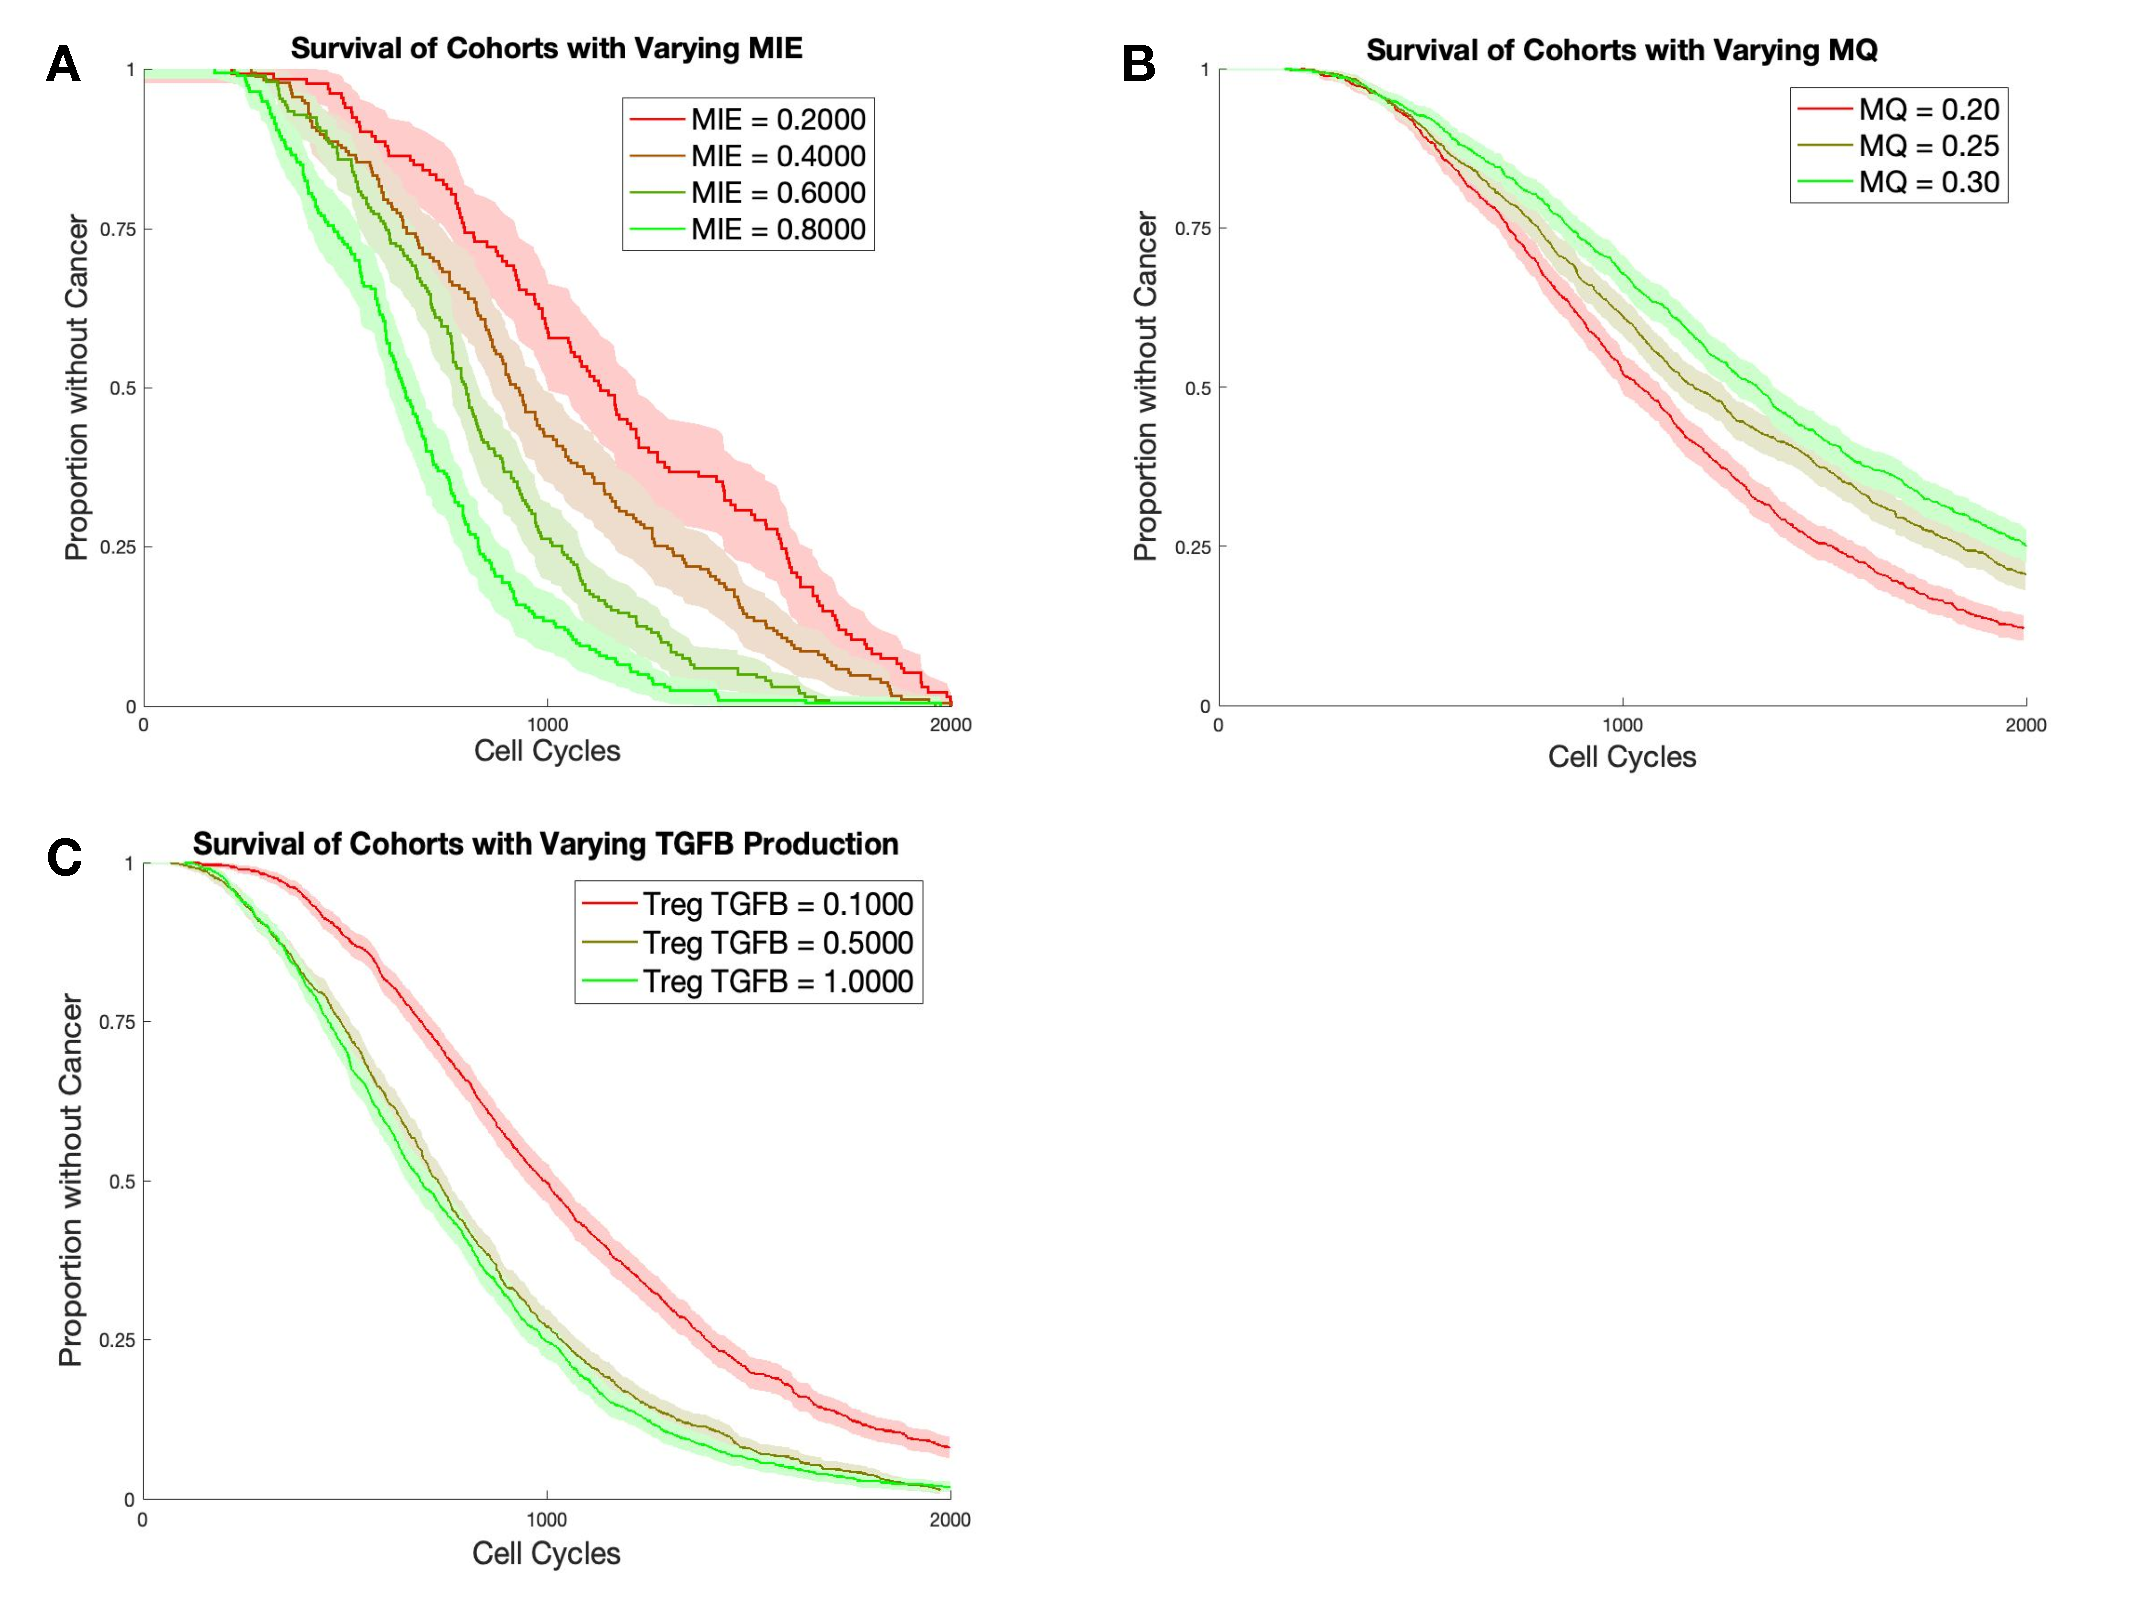
\includegraphics[width=\columnwidth]{Figure2/Figure2.pdf}}
\caption{
A. Increasing MIE decreases Time to Cancer. 
B. Increasing MGA increases Time to Cancer.
C. Increasing Treg TGF-$\beta$ production results in decreased Time to Cancer.
%% {\color{red} Cox regression or KM test statistics to be computed to demonstrate the significance of this claim.}
}
\label{fig:FirstSurvivalCurves}
\end{figure}

Second, as mesenchymal growth arrest (MGA) increases, Time to Cancer increases.
This result will prove to be more interesting as this pattern is dependent on the other parameters in the model.
For now, what can be seen in Figure \ref{fig:FirstSurvivalCurves}B is that a slower proliferation for mesenchymal cells slows down cancer growth.
This is not as intuitive as it may sound because this decreased proliferation affects both mutated and non-mutated cells.
% It may be interesting to track how much MGA affects mutated vs. non-mutated cells throughout the time.
These results are summarized by Figure \ref{fig:FirstSurvivalCurves}B.

Third, TGF-$\beta$ can be varied in two ways: the production by mesenchymal cells and the production by Treg cells.
In Figure \ref{fig:FirstSurvivalCurves}C, the results of varying Treg TGF-$\beta$ production is shown, indicating that an increased Treg TGF-$\beta$ production leads to a shorter Time to Cancer.
This is expected as the two main ways in which TGF-$\beta$ influences the system is in recruitment of Treg cells and in pushing tissue cells to a mesenchymal phenotype.
Treg cells are modeled as tumor-protective and thus increasing their number will naturally decrease Time to Cancer.
Mesenchymal cells are more likely to evade the immune system, so pushing the system towards an overall more mesenchymal phenotype will better protect the cancer and decrease the Time to Cancer.
% But what happens when MIE is really high to begin with so becoming mesenchymal mostly just makes you proliferate slower? Perhaps that can go in a supplementary figure?

\subsection{Key EMT regime maximizes cancer-free survival time under chronic inflammation}\label{KeyEMT}
Given the relevance of the inflammatory state of the tumor microenvironment (TME), we explore the effect of varying the inflammation state of the patient on survival.
In particular, some cohorts are assigned permanently low inflammation, others permanently high, and still others non-constant inflammatory schemes.
For those cohorts with a permanently high inflammatory state, the relationship between the mesenchymal parameters and the Time to Cancer is monotonic.
However, when there are periods of a low inflammatory state, then intriguingly the connection between MGA and Time to Cancer becomes concave down with a local maximum around 0.3.
This can be seen in the top two groups of Figure \ref{fig:VaryINFL_and_MesPars}D in which the MGA=0.3 cohorts both took longer to cancer than their neighbors.
What this indicates is that if the growth arrest of mesenchymal cells can be controlled, then they could be manipulated in such a way as to increase the Time to Cancer.
Furthermore, even if the patient is presenting a permanent high inflammatory state, medications could be prescribed which would lower the inflammatory state temporarily and thus create a similar cycling inflammatory regime which could be taken advantage of in the same way.
% A Is this next sentence necessary?
% AM: can remove it 
See Figure \ref{fig:VaryINFL_and_MesPars}C and Figure \ref{fig:VaryINFL_and_MesPars}D for a summary.

\begin{figure}[H]
\center
\frame{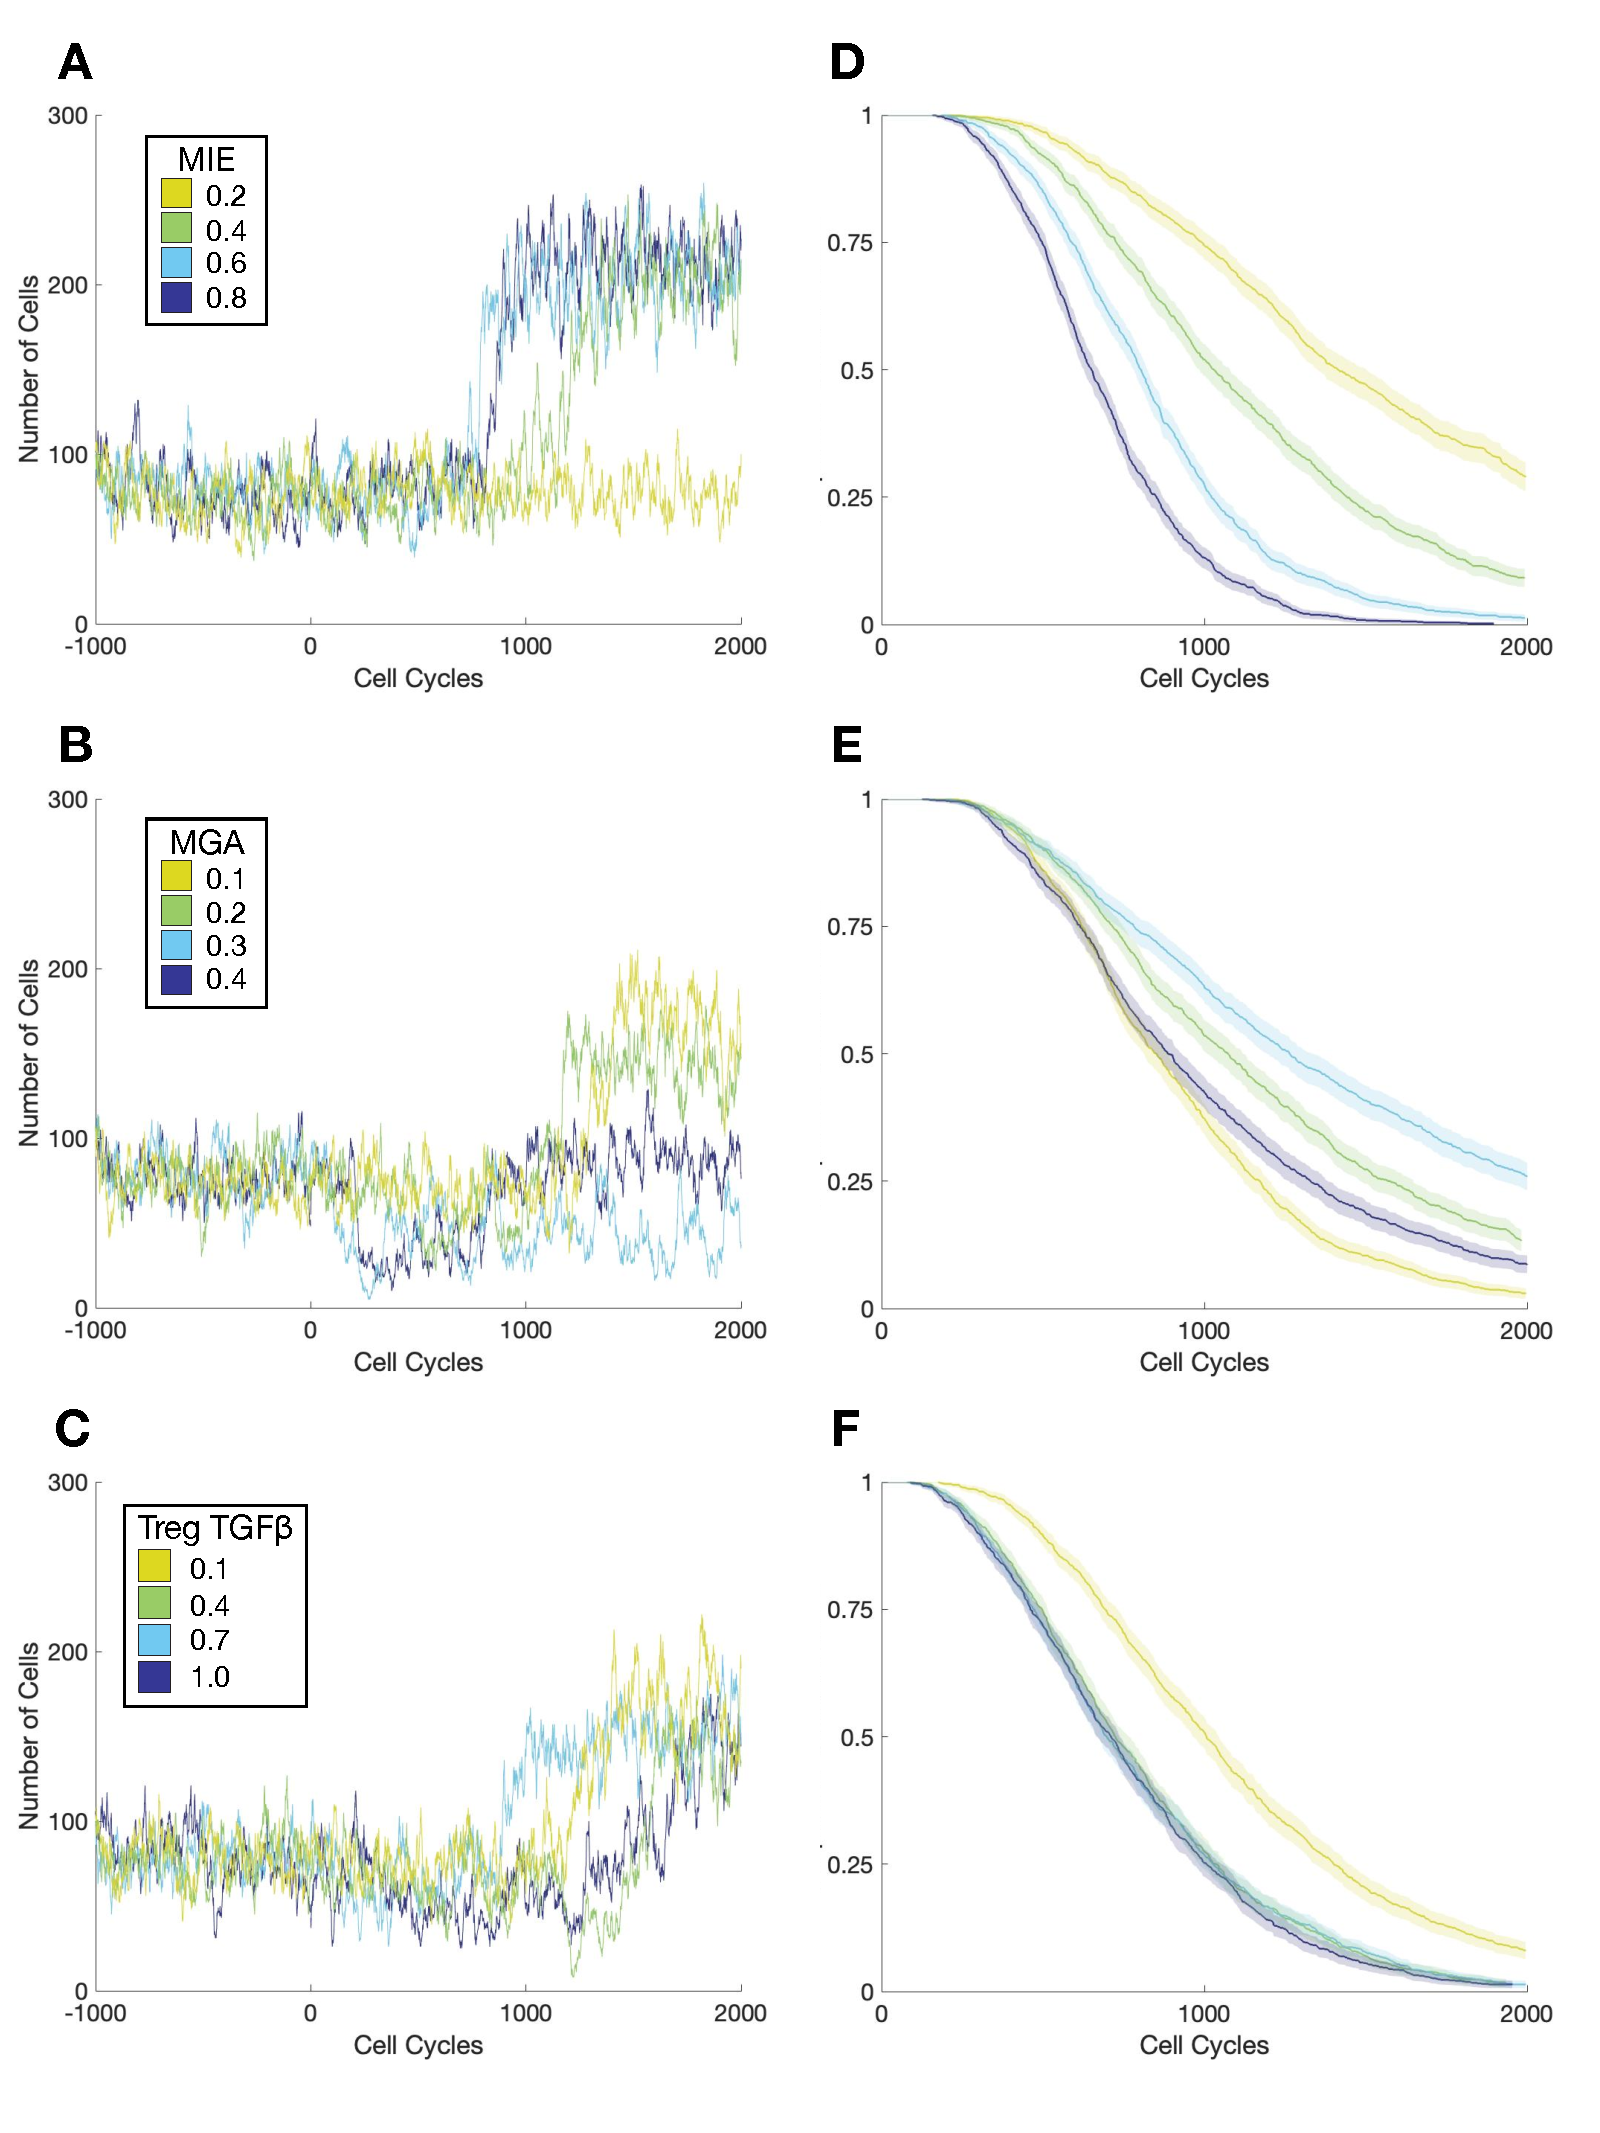
\includegraphics[width=\columnwidth]{Figure3/Figure3.pdf}}
\caption{A.Survival curves for various inflammation cycling schemes. In the top two plots, the Time to Cancer decreases as MIE increases. In the bottom plot, there is no significant difference in survival.
B. The average Time to Cancer for each cohort.
C. Survival curves for various inflammation cycling schemes. In the top two plots, the Time to Cancer reaches a maximum value somewhere near MGA = 0.3. In the bottom plot, there is no significant difference in survival.
D. The average Time to Cancer for each cohort.}
\label{fig:VaryINFL_and_MesPars}
\end{figure}

Contrast this with what happens when MIE is varied for different inflammation cycling schemes.
Regardless of the cycling scheme, the relationship between Time to Cancer and MIE is always -monotonic.
In the case that the inflammatory state is permanently high, MIE has no significant effect on Time to Cancer.
On the other hand, when the patient experiences at least some time in a low inflammatory state, an increase in MIE results in a decrease in Time to Cancer.
This indicates that mitigating a chronic inflammatory state is a necessity for increasing survival, and once that has been achieved, even to a small degree, then therapies which reduce mesenchymal immune evasion will gain efficacy.
% A Is this next sentence necessary?
% AM: remove
See Figure \ref{fig:VaryINFL_and_MesPars}A and Figure \ref{fig:VaryINFL_and_MesPars}B for a summary.

\subsection{Heat Map of MIE vs MGA}
To further draw out the contrast between these two mesenchymal properties, we compare Time to Cancer for many different pairs of values for MIE and MGA.
The heat map in Figure \ref{fig:MIEvsMGA} concisely encodes the relationships we have been observing in the previous sections.
Regardless of the value of MGA, increasing MIE leads to decreased Time to Cancer.
On the other hand, for any value of MIE, then there is an MGA value that results in the longest Time to Cancer.
For the model, this optimal value increases with MIE.

\begin{figure}[H]
\center
\frame{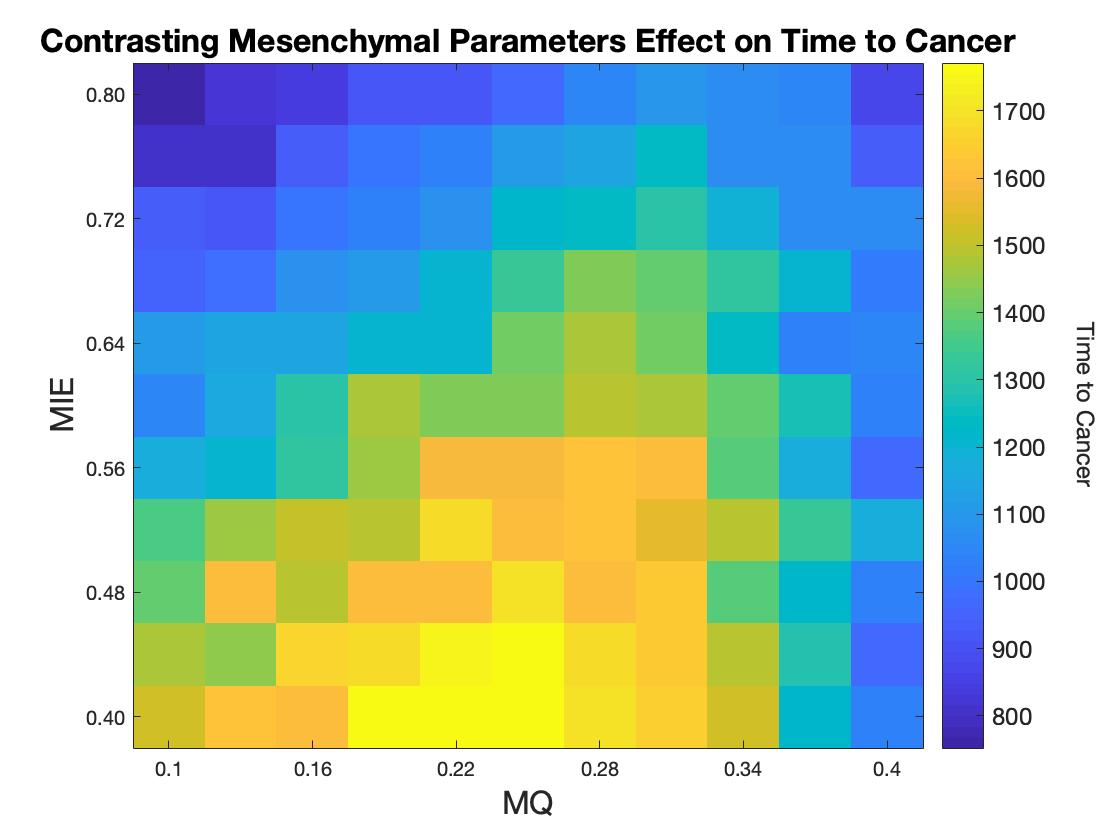
\includegraphics[width=\columnwidth]{Figure4/MIEvsMQ.jpg}}
\caption{Heat Map contrasting the effects of MIE and MGA on Time to Cancer. Increasing MIE always decreases Time to Cancer, but MGA is non-monotonically linked to Time to Cancer.}
\label{fig:MIEvsMGA}
\end{figure}

%%%%%%%%%%%%%%%%%%%%%%%
%                      DISCUSSION                       %
%%%%%%%%%%%%%%%%%%%%%%%

\section{Discussion}\label{Discussion}
In building this model, we set out to better understand how the immune system and the EMT spectrum would affect Time to Cancer results from previous work.
What we found is that altering many of the processes have predictable results: increasing mesenchymal immune evasion, decreasing mesenchymal growth arrest, and increasing Treg TGF-$\beta$ production all lead to shorter Times to Cancer.
However, when the inflammation of the TME is accounted for, some of these changes to the system have less predictable outcomes.
The most intriguing is that periods of low inflammation lead to mesenchymal growth arrest having an optimal value for maximizing Time to Cancer.



%In addition, I could discuss the implications from the TGF-$\beta$ section.
%Any discussion on this topic, however, would need to acknowledge that regulation of TGF-$\beta$ might also have other, serious side effects, especially if the treatment is not local.
%However, that might also be true for the inflammatory results.
%In light of this, it might be good to include a new section on how TGF-$\beta$ production's influence on Time to Cancer is influenced by the inflammatory cycling scheme.



%%%%%%%%%%%%%%%%%%%%%%%
%                     CONCLUSION                      %
%%%%%%%%%%%%%%%%%%%%%%%

\section{Conclusion}\label{Conclusion}
The interactions of the immune system and cancer remain a promising avenue of research.
Including more diverse aspects of the TME and the tumor itself make the challenge that much harder but also that much more promising.
As we begin to understand how processes such as EMT factor in to these complex interactions, we can begin to respond clinically to better improve patient outcomes.
Here, we saw {\it in silico} evidence of an optimal value for a property of mesenchymal cells that would maximize Time to Cancer.
There is still much work to be done further isolating this effect in computer simulations and further verifying this effect and exploring further ways EMT can influence tumor progression.
This model explored much more than mesenchymal growth arrest, so a simpler model could make this point clearer.
On the other hand, models which incorporate more distinctions between epithelial and mesenchymal cells could give better clarity on the relative importance of these and reveal a fuller picture about how a mesenchymal subpopulation affects cancer outcomes.

%A Adam, do you know of any?
The authors are not aware of current treatments that specifically target mesenchymal growth arrest, influencing it in one direction or another.
%
Based on these results, this could prove to be a promising direction for research, in particular for cancers in which it is known that mesenchymal cells are present and active within the tumor.
The greatest challenge in translating the information here to the clinic, apart from creating the drugs, would be discovering the ideal growth rate for mesenchymal cells within each patient and how other patient-specific data will influence this result.

Progress in cancer treatment has always proven attainable even despite great challenges, for which the complexity of the disease is often responsible. As we move forwards, it is these very complexities that we will be able to better exploit to eradicate or control the disease.


\bibliography{mybib}{}
\bibliographystyle{siam}

\end{document}